%% LaTeX2e Supplemential Instruction Template by Stephen Iota (https://stepheniota.com/)
%% last updated: May 2019
\documentclass[11pt]{article}
\usepackage[margin=2.5cm]{geometry}
%%%%%%%%%%%%%%%%
%%% Packages %%%
%%%%%%%%%%%%%%%%
\usepackage[utf8]{inputenc}
%\usepackage{lipsum}
\usepackage{amsmath,amssymb,amsfonts,physics}
\usepackage{graphicx}
\usepackage[shortlabels]{enumitem}
\usepackage[dvipsnames]{xcolor}
%\usepackage{footmisc}
\usepackage[small]{titlesec}
%\usepackage{fancyhdr}
\usepackage[
	colorlinks=true,
	citecolor=NavyBlue!90!black,
	linkcolor=NavyBlue!75!black,
	urlcolor=green!50!black,
	hypertexnames=false]{hyperref}
 %%%%%%%%%%%%%%%%%%
 %% New Commands %%
 %%%%%%%%%%%%%%%%%%
\newcommand{\email}[1]{\texttt{\href{mailto:#1}{#1}}}
%%%%%%%%%%%%%%%%%%
%% Front Matter %%
%%%%%%%%%%%%%%%%%%
\pagenumbering{gobble} % no page numbers
\graphicspath{{figures/}} % set directory for figures
\setcounter{section}{-1} % start with section 0
%%%%%%%%%%%%%
%%% Title %%%
%%%%%%%%%%%%%
\begin{document}
\begin{center}
\Large{\textsc{PSet 5}: \textbf{Superposition \& standing waves}}
\end{center}
\vspace{.5mm}
%%%%%%%%%%
%% INFO %%
%%%%%%%%%%
\begin{tabular}{rl}
\textsc{SI Leader}:			& 			Stephen Iota (\email{siota001@ucr.edu})
\\
\textsc{Course}:				&			Physics 40B (Spring 2019), Prof.~Barsukov
\\
\textsc{Date}:					&			\today
\end{tabular}
%%%%%%%%%%%%%%
%% PROBLEMS %%
%%%%%%%%%%%%%%


\section{Investigating the principle of superposition}

Explain the principle of superposition.
Now, construct two wave fronts traveling towards each other with a specified velocity for each.
Draw the initial snapshot graph.
Next, elapse the system for some time until the two wave fronts.
Draw another snapshot graph at the new time, paying special attention to how the two waves interfere with each other.


\section{Resonances in open-closed tubes}

\begin{figure}[h!]
\centering
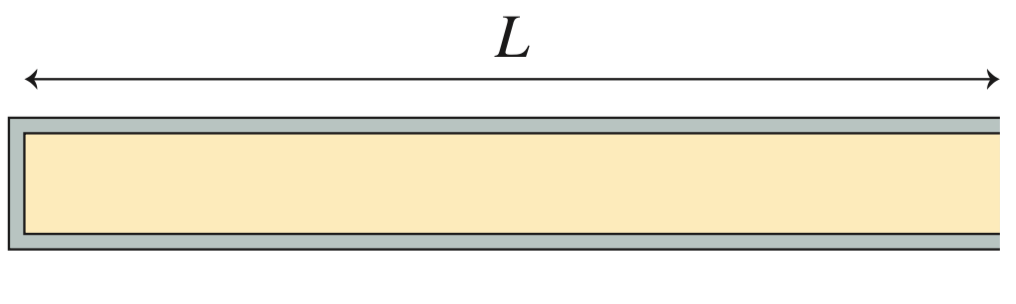
\includegraphics[width=.4\linewidth]{PSet5_Fig1}
\caption{Open-closed tube of length $L$.\label{tube}}
\end{figure}
\\
\noindent
Let's think about what allowed modes of sounds waves are allowed in an open-closed tube such as in figure~\ref{tube}.
\begin{enumerate}[(a)]
\item Propose a general formula for the allowed wavelengths $\lambda_n$ and frequencies $f_n$ which generate standing waves in the open-closed tube.
\item How do the boundary conditions for this system differ from the closed-closed system discussed in lecture?
\end{enumerate}



\section{Wave reflection}

Consider a string with a large linear density is connected to one with a smaller linear density. A wave packet is traveling from the string with higher density to the string with lower density.
\begin{enumerate}[(a)]
	\item What will the wave speed be once the wave packet crosses the discontinuity?
	\item Does part of the wave packet get reflected at the discontinuity? If so, what is the phase shift of the reflected wave?
	\item Draw the transmitted and reflected wave packets with appropriate phase shifts.
\end{enumerate}
Now, consider the opposite scenario. A wave packet is traveling through a string with low linear density and reaches a string with large linear density. Repeat parts (a) -- (c) for this case.

\end{document}
